\documentclass[a4paper]{article}

\usepackage[english]{babel}
\usepackage[utf8x]{inputenc}
\usepackage{amsmath}
\usepackage{graphicx}
\usepackage[absolute,overlay,showboxes]{textpos}
\usepackage{xcolor}
\usepackage{float}
\usepackage{pgfgantt}
\usepackage[colorinlistoftodos]{todonotes}

\setlength{\TPHorizModule}{1mm}
\setlength{\TPVertModule}{1mm}


\title{Plan de rapport de stage de Guillaume Maitrot }
\author{Guillaume Maitrot}


\begin{document}

\begin{titlepage}

\begin{textblock}{110}(0,0)

\includegraphics[width=0.47\textwidth]{38040_logo-trans.png}

\end{textblock}

\begin{textblock}{100}(110,0)

\includegraphics[ width=1.5\textwidth]{logo_ircica-transparent-mini-2.png}
\end{textblock}



\begin{textblock}{220}(0,100)
\centering
\title{RAPPORT DE STAGE}
\author{Guillaume Maitrot}
\date{Avril à Juin 2016}
\maketitle
\title{Stage de Licence 3 Informatique}
\maketitle
\paragraph{}
\end{textblock}


\centering
\begin{textblock}{220}(0,200)
\paragraph{Tuteur en entreprise : Julien Forget}
\paragraph{Tuteur académique : Vincent Hugo }
\paragraph{Etablissement : Université Lille 1 /Licence informatique }
\paragraph{Entrerpise d'acceuil : Ircica }
\paragraph{}
\end{textblock}


\end{titlepage}


\section{Remerciements}

\begin{itemize}
\item{Julien Forget : Maître de Conférences - Université de LILLE1.} Pour son aide quotidienne à l'apprentissage de la carte stm32 et du temps réel. 
\item{Giuseppe Lipari : Professeur des Universités de LILLE.} Pour son aide à la compréhension de la FFT et des résultats. 
\item{Alexandre Boé : Maître de Conférences - Université de LILLE1.} Pour le côté électronique et le matériel.
\item{Thomas Vantroys : Maître de Conférences - Université de LILLE1.} Pour son aide à la compréhension des périphériques de la carte STM32. 
\item{Nadir Cherifi : Doctorant.} Pour son aide avec le système de fichier et l'utilisation de ses scripts avec un analyseur de puissance, l'Agilent N6075. 
\item{Tilen Majerle : un ingenieur en recherche et développement qui a travaillé sur la carte stm32.} Pour ses exemples de code d'utilisation de la carte stm32. 
\end{itemize}



\begin{titlepage}

\section{Sommaire}

\tableofcontents


\end{titlepage}

\section{Introduction}

\section{Présentation de l'entreprise}

\subsection{Qu'est-ce IRCICA}
L'institut de Recherche en Composants logiciels et matériels pour l'Information et la Communication Avancée (IRCICA) associe le CNRS (Centre National de la Recherche Scientifique) l'Université Lille1. Il rassemble près de 120 membres provenant de quatres différents laboratoires. Voici plusieurs axes de recherche :



\begin{itemize}
\item Les interfaces homme-machine. 
\item Les réseaux de capteurs. 
\item La photonique. 
\item Les architectures bio-inspirées.
\end{itemize} 
     

L'IRCICA fonctionne comme un ‘hôtel à projets’, l’IRCICA associe environ 120 enseignants-chercheurs, chercheurs, étudiants, ingénieurs et techniciens de quatre laboratoires partenaires : l’IEMN, le LIFL, le Phlam, le L2EP .

La politique scientifique de l’IRCICA vise à initier des projets de recherche interdisciplinaires associant les différentes communautés présentes dans l’institut, en particulier celles du matériel et du logiciel.
Les projets en cours concernent les nouveaux dispositifs photoniques, les réseaux autonomes ultra faible énergie, les interfaces tactiles haptiques et les architectures bio inspirées de traitement de l’information.

\subsection{Le projet WhatTheWatt}
Le projet WhatTheWatt est la suite d'un autre projet qui était WattSoft. Ces deux projets ont été crée car le nombre de systèmes embarqués fonctionnant sur batterie croit rapidement dans de nombreux domaines de l'informatique embarquée pour ce faire ils vont essayer de modéliser la consommation d'énergie de logiciel temps réel embarqué. Avec l'aide d'études récentes montrent que réel montre que la consommation du système est modélisée sur la base quasiment exclusive des caractéristiques physiques de la plateforme et que la seule caractéristique logicielle prise en compte est en fait la durée d’exécution des tâches logicielles. Les projets IRCICA SY-NERGIE et WattSoft ont montré qu’un tel modèle est peu réaliste, en particulier pour des petites plateformes à faible puissance de calcul, dans lesquelles la consommation varie de manière importante selon l’utilisation des périphériques (stockage de données, communication réseau, etc) et la nature des traitements exécutés (calculs arithmétiques, branchements, accès mémoire, etc). L’objectif de WattSoft était de comprendre pourquoi le logiciel consomme, en analysant les instructions exécutées, l’utilisation des périphériques, etc. L’objectif de WhatTheWatt sera de comprendre comment le logiciel consomme, c’est-à-dire d’obtenir une représentation de la consommation de ce logiciel, au lieu d’analyser pourquoi on obtient cette consommation. Les étapes prévues pour la réalisation de ce projet sont les suivantes : 

\begin{itemize}
\item Implémentation d’applications sur carte embarquée fonctionnant avec un système d’exploitation temps réel (FreeRTOS). Les applications candidates sont le serveur web minimaliste SMEWS (développé par 2XS) ainsi que des benchmarks embarqués classiques de traitement du signal (type FFMpeg);

\item Mesure de la consommation de ces applications. L’objectif sera ensuite d’obtenir une représentation mathématique de ces mesures : constante au cours du temps, affine, ou autre. Le choix de cette représentation sera le résultat d’un compromis entre le fait qu’elle doive être réaliste, c’est à dire proche de la réalité mesurée, tout en restant exploitable par un système d’exploitation dont l’objectif serait de réduire la consommation du système embarqué;

\item Mesure de la consommation de plusieurs applications exécutées en concurrence sur une même plateforme matérielle. L’objectif sera ici de mesurer l’impact des interférences entre ces applications.
\end{itemize}

Le projet WhatTheWatt est une coopération de plusieurs équipes d'Ircica,Julien Forget le coordinateur du projet, Giuseppe Lipari, deux stagiaires Guillaume Maitrot et Corentin Casier pour l'équipe Emeraude, Thomas Vantroys pour l'équipe 2XS et Alexandre Boé pour l'équipe CSAM. 
A moyen terme, c’est-à-dire dans le cadre du projet IRCICA, notre travail permettra d’obtenir une caractérisation chiffrée de la consommation d’énergie d’un composant logiciel embarqué temps réel au fil de son exécution. Cette caractérisation sera basée uniquement sur la mesure et non sur l’analyse du code des applications ciblées. A plus long terme, nous espérons proposer des politiques d’ordonnancement adaptées au modèle défini dans ce projet et les intégrer dans des systèmes d’exploitation destinés à l’embarqué, tels que FreeRTOS, Erika ou Linux.

\section{Présentation du stage}

\subsection{Sujet du stage}

Le but de mon stage est de mesurer la consommation du processeur et périphériques d'une application simple de traitement du signal d'une carte embarquée par le biais d'un analyseur de puissance l'Agilent N6705 qui va mesurer une simple application de traitement de signal qui se résume à prendre une donnée par le convertisseur numérique à la transformer avec la FFT (Fast Fourier Tranformation, sert à convertir des données de courant en données de fréquence), puis à écrire les résultats sur la carte mémoire flash, pour ainsi voir quel périphérique de la carte stm32 consomme le plus et ainsi pouvoir réduire la consommation du code dans les systèmes embarqués en général. 


\subsection{Le contexte de mon travail}

 Mon stage a commencé le 4 avril 2016 pour finir le 1 juillet 2016 pour l'équivalent de 13 semaines. Il nécessitait des connaissances en programmation bas niveau en C sur carte embarquée. Pour faire mon stage j'ai eu besoin de divers matériels.

 \begin{itemize}
 
\item Une carte STM32f4-discovery avec un ARM Cortex -M4 32-bit (voir la figure ~\ref{fig:Carte}). J'ai utilisé sur cette carte les pattes d'entrées et de sorties situé sur la partie gauche et droite de la carte qui m'ont servi de connexion entre la carte et les périphériques, un bouton noir "reset" pour relancer le code, ainsi que quatre LED en dessous du processeur pour commencer à apprendre à utiliser la carte et elles m'ont aussi servi dans le débugage, car grâce à elles je pouvais voir quand le code s'arrêtait de s'exécuter et d'un port d'usb d'alimentation et de connexion entre la carte et l'ordinateur pour envoyer le code désiré dans la carte et aussi pour l'alimenter. 
 
 \begin{figure}[!ht]
\centering
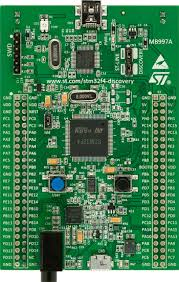
\includegraphics[width=0.8\textwidth]{index.jpeg}
\caption{\label{fig:Carte}Photo de la carte stm32F4-discovery}
\end{figure}
  
\item Ainsi qu'un générateur de basses fréquences, un outil qui va donner une tension avec une fréquence définie.

\item Une carte mémoire flash qui va servir comme support pour les résultats donnés par l'application simple.

\item Mais aussi un Agilent qui est un analyseur de puissance (voir la figure ~\ref{fig:Agilent} ), l'outil qu'on va utiliser pour mesurer la consommation des tâches. Il possède quatre voies qui peuvent servir d'alimentation et/ou de canal de mesure qu'on peut voir en bas à droite de l'image, ainsi qu'un menu où on peut régler le courant et l'intensité de chaque voie, un oscilloscope qui permet de voir l'intensité, le courant de chaque courbe résultant d'une des voies, l'écran peut se changer en menu ou en oscilloscope. Avec les molettes en bas à gauche on peut changer l'unité de mesure de l'intensité ou de courant propre à chacune des courbes, mais aussi de leurs données une adresse de manière relative pour ainsi concentrer les courbes dans un espace restreints afin de toutes les voir en même temps sans changer leur valeur, on peut également changer l'unité de mesure du temps, mais pour toutes les courbes. 

\begin{figure}[!ht]
\centering
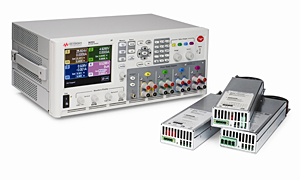
\includegraphics[width=1\textwidth]{N6705A_4_2007Mar5-300x180.jpg}
\caption{\label{fig:Agilent}Analyseur de puissance l'Agilent N6705}
\end{figure}

\item Mais également d'une BreadBoard (voir la figure ~\ref{fig:BreadBoard} ) qui permet de faire des schémas d'électroniques sans à avoir à souder les composants ensemble. Tous les composants réunis sur une ligne d'un côté uniquement sans les colonnes rouges et bleu sont connectés ensemble, le positif ici la colonne rouge est relié par bloc de 5, de même pour la colonne des négatifs ici celles en bleu. On peut bien sûr brancher des fils pour créer une connexion entre lignes ou colonne.  

\begin{figure}[!ht]
\centering
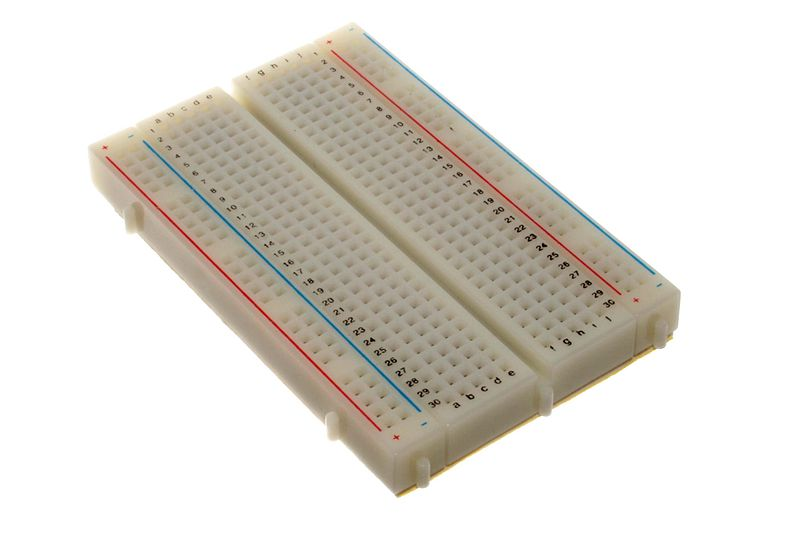
\includegraphics[width=0.5\textwidth]{breadboard.jpg}
\caption{\label{fig:BreadBoard}photo d'une BreadBoard}
\end{figure}

\end{itemize}


\subsection{La répartition du temps de mes tâches}

\begin{ganttchart}[vgrid=*1{red, dotted},hgrid=*1{black ,dotted}, link mid=0.4]{1}{13}
\gantttitle{2016}{13} \\
\gantttitle{Avril}{4}
\gantttitle{Mai}{5}
\gantttitle{Juin}{4}\ganttnewline
\gantttitlelist{1,...,13}{1} \\
\ganttbar{Prise en main de la plateforme}{1}{2} \\
\ganttlinkedbar{Programmation des périphériques}{3}{3}\ganttnewline
\ganttlinkedbar{Développement de l'application}{4}{4}\ganttnewline
\ganttlinkedbar{Programmation multi-threadée}{4}{5}\ganttnewline\ganttlinkedbar{Mesure de la consommation}{6}{9}\ganttnewline
\ganttlinkedbar{écriture du rapport}{10}{10}\ganttnewline
\ganttlinkedbar{préparation de la soutenance}{11}{11}\ganttnewline
\ganttlinkedbar{Etude des variations}{12}{13}
\end{ganttchart}


\section{Travail effectué au cours de mon stage}

\subsection{Prise en main de la plateforme : compilation de code C pour la carte STM32, découverte de FreeRTOS. }
Quand j'ai commencé mon stage je n'avais que très peu vu les systèmes embarqués, alors pour commencer je devais tout d'abord faire que le projet de mon prédécesseur compile qu'il soit donc compatible avec mon ordinateur, installer les paquets nécessaires au projet. Après que j'ai réussi à compiler le code de mon prédécesseur j'ai regardé le makefile pour savoir la structure et l'organisation du projet. Avec des explications fournies j'ai pu créer un petit code de test ne faisant rien et l'envoyer dans la carte. Grâce à ça j'ai appris à envoyer le code sur la carte stm32, ensuite je décidais de créer un code pour faire clignoter une led, j'ai dû chercher sur internet des tutoriels de comment allumer une led, et avec l'aide du tutoriel et d'un code déjà existant dans le projet j'ai réussi à faire clignoter la led verte sur la carte STM32. Tout ceci étant fait en baremetal je devais aussi réussir à faire un clignotement de led sur FreeRTOS, ce ne fut pas difficile avec un exemple déjà fait, grâce à celui-ci j'ai appris à utiliser des fonctions primaires de FreeRTOS comme le délai, la création des threads qui sont une séquence d'instructions qui s'exécutent parallèlement aux autres threads et également comment lancer les threads sous FreeRTOS.

Je n'avais jamais eu besoin de faire une initialisation d'une partie de la carte, mais grâce aux exemples j'ai pu apprendre facilement comment initialiser les différents composants interne du microcontrolleur de la carte pour ainsi l'utiliser dans le code. Je n'avais pas l'habitude de faire un délai moi-même ainsi que ne pas utiliser des fonctions aussi primaires. J'ai dû m'adapter, par exemple pour le délai je faisais un certain nombre d'actions inutiles coûtant du temps pour attendre.

Le but de cette tâche était de me familiariser avec la carte STM32 et son fonctionnement d'abord on crée un projet avec un fichier en langage c, main.c ensuite on le compile pour que le code fonctionne avec le projet puis ensuite on l'envoie sur la carte pour qu'il s'exécute et aussi de commencer à utiliser un os minimaliste, avec peu de fonctions.


\subsection{Programmation des périphériques de la carte.}

Pour pouvoir utiliser l'usart qui fait la liaison entre l'ordinateur et un port série de la carte STM32F4-discovery et on m'a donné un ftdi basic de Sparkfun qui permet la communication entre la carte et l'ordinateur, j'ai dû l'initialiser dans le programme puis commencer à le tester, après quelques tests j'ai remarqué que sans délai on n'était pas sûr du résultat donné par l'usart il pouvait passer au symbole suivant sans avoir écrit son symbole actuel, car sa vitesse était trop lente par rapport à l'envoi des données.

Il avait déjà un exemple de convertisseur analogique-Numérique sur le projet, mais incomplet pour que je l'utilise directement dans l'application simple, il manquait la conversion, il prenait seulement la donnée transmise sur une des pattes d'entrée/sortie de la carte STM32 connecté à la ftdi basic connecté à un minicom qui permettait la communication entre mon ordinateur et la ftdi.

Ensuite, après avoir juste reçu la donnée on doit la convertir, Alexandre m'a dit tout d'abord d'essayer d'utiliser le capteur de température de la carte STM32 pour savoir la température du processeur. J'ai pu ainsi faire un test pour voir si effectivement la conversion fonctionnée en ayant la température du processeur. Le test m'a donné comme résultat la figure~ref{fig:mesureTemperature}, on peut voir sur ce schéma que la température du processeur avoisine les 30 dégrées, ce qui est cohérent avec une température du processeur. 

\begin{figure}[H]
\centering
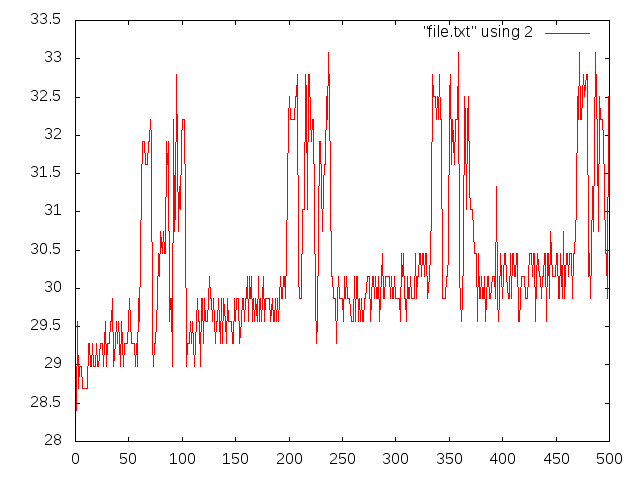
\includegraphics[width=1\textwidth]{test_temp.png}
\caption{\label{fig:mesureTemperature}Courbe de mesure de la température du processeur en dégrée par rapport à son numéro d'échantillon}
\end{figure}

Il fallait ensuite tester voir si la conversion du courant était correct. Pour cela il fallait prendre un des canaux du convertisseur Analogique-Numérique pour brancher une entrée de courant. Pour le test il fallait deux valeurs sûr j'ai donc testé pour 0V et 3V qui pour 0V était la valeur la plus faible dans la conversion et 3V qui était la valeur la plus forte. Comme le résultat était en hexadécimal pour la valeur la plus faible il fallait 000 car le convertisseur sort des données sur douze bits et un caractère hexadécimal en prenait quatre, donc trois caractères, mais aussi FFF pour la valeur la plus forte ici 3V. Après que j'ai branché le canal du convertisseur à une entrée à 0V (la masse), le résultat était d'environ en hexadécimal 000, pour l'entrée à 3V il sortait FFF en hexadécimal.

Après ces vérifications j'ai dû m'attaquer au problème de l'écriture dans la carte mémoire flash, grâce à l'aide de Nadir Cherifi qui m'a montré les branchements de connexion entre la carte STM32 directement sur un adaptateur SD, ou un shield contenant la carte SD. Avec la compilation du code de Tilen Majerle pour le système d'exploitation de fichier, la FAT, j'ai pu écrire un morceau de texte dans la carte mémoire, même s'il y avait encore quelque problème d'alimentation entre la carte STM32 et la carte mémoire flash, car il faut parfois appuyer plusieurs fois sur le bouton reset pour que le code s'effectue.

Je ne savais pas comment configurer le minicom qui est un programme de contrôle de modem et d'émulation de terminal, qui ici servait à la communication entre l'ordinateur et la carte stm32, grâce à cette communication je vais pouvoir l'utiliser pour m'envoyer des données quand un code ne marchera pas ou ne s'exécute pas correctement pour le débuger.

L'adc soit le convertisseur Analogique-Numérique avait déjà un code existant dans le projet, mais il manquait la conversion. J'ai donc dû chercher sur le net la conversion appropriée, il en existait plusieurs, mais une seule convenait à la fiche technique de la carte STM32.

Sans les accès d'un os je ne savais pas comment accéder à la mémoire d'une carte mémoire flash, mais grâce à un système d'exploitation de fichier : la FAT j'ai pu écrire et lire dans la carte mémoire flash. 

Grâce à l'apprentissage d'utilisation de l'usart en port série je vais pouvoir avec plus de facilité à débuger mes programmes et avec le convertisseur et l'écriture sur la carte mémoire commencer une partie de l'application.  


\subsection{Développement de l'application simple. }

Après avoir fait des tests sur des entrées constantes pour le convertisseur Analogique-Numérique (0V et 3V), on m'a donné un GBF (générateur de basses fréquences) qui va donner des données de courant en sinusoïdales, mais aussi une fréquence accordée à celle-ci, il va nous permettre d'avoir une réel entrée de courant qu'une constante pour que la tâche de la conversion soit plus réaliste. J'ai découvert aussi la FFT qui avec une courbe d'entrée de courant nous donne son signal de fréquence.

J'ai dû avant tout de vérifier que le générateur de basse fréquence était connecté à la carte STM32 et que la conversion était juste, pour cela je devais obtenir une sinusoïdale entre 0V et 3V. On voit sur la figure ~ref{fig:mesureDEntree} qu'on obtient bien une sinusoïdale entre 0V et 3V, cette sinusoïdale résultant d'une écriture des données converties par le convertisseur Analogique-Numérique dans un fichier qui sera ensuite affiché par gnuplot qui est une interface pour la représentation graphique de données provenant d'un fichier texte.

\begin{figure}[H]
\centering
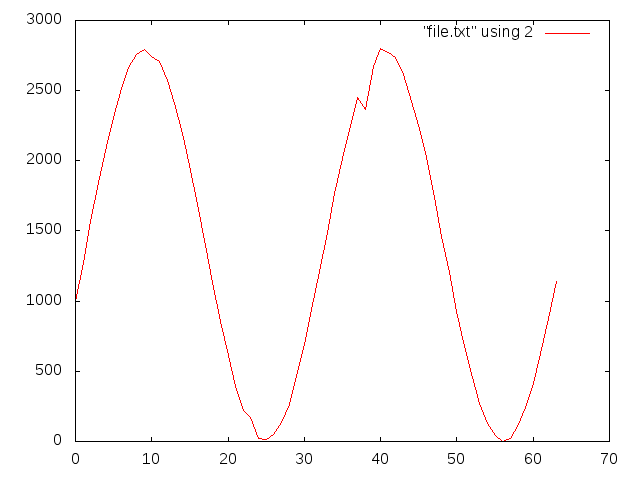
\includegraphics[width=0.8\textwidth]{input.png}
\caption{\label{fig:mesureDEntree}Courbe de mesure du courant du Générateur basse fréquence en MV par raport à son numéro d'échantillon}
\end{figure}

Mais aussi que quand nous changeons la fréquence du générateur basse fréquence, nous obtenons des courbes différentes mais cohérentes, sur la figure ref{fig:mesureDEntree} on peut calculer 8HZ, grâce aux données suivantes : une période prend le temps d'environ 32 échantillons et un échantillon se mesure tous les quatre millisecondes, cela nous fait pour une période une durée de 128 ms, on sait que le temps de la période et la fréquence est reliée par la relation fréquence = 1/ temps de la période où le temps est en seconde et la fréquence en HZ. Cela nous fait donc 1 /0.128 qui équivaut environ à 8HZ. Suivant cette logique on peut déduire que pour 16HZ on aura un temps de période équivalent environ à 62.5 ms soit un peu moins de 16 échantillons et on peut voir sur la figure ~ref{fig:comaparaison1} qu'une période prend environ 16 échantillons.
                                                                             
\begin{figure}[H]
\centering
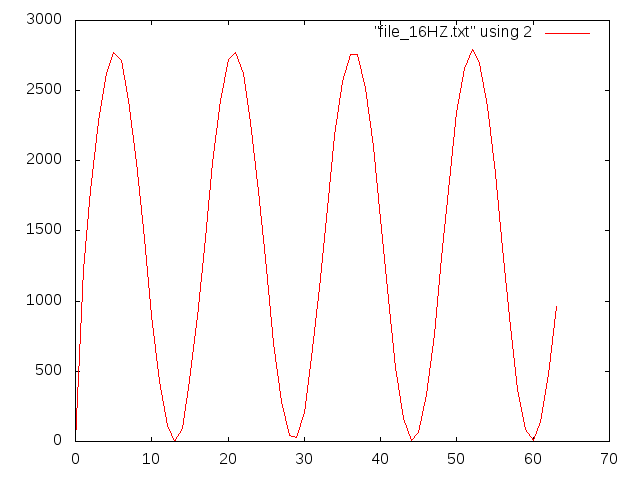
\includegraphics[width=0.95\textwidth]{input16HZ.png}
\caption{\label{fig:comaparaison1}Courbe de mesure du courant du Générateur basse fréquence à 16 HZ en MV par raport à son numéro d'échantillon}
\end{figure}

Pour effectuer cette tâche, j'ai dû apprendre à utiliser une FFT (Fast Fourier Tranformation) qui sert à convertir des données de courant en données de fréquence qui va être une des tâches de l'application simple et à comprendre comment l'utiliser et ainsi donc mettre les données de sorties du convertisseur Analogique-Numérique dans la FFT puis écrire ces résultats dans la carte mémoire flash via le système de fichier FAT qui sera la tâche finale de l'application simple. J'avais obtenu un résultat  de l'application simple cohérent avec les attentes, mais il restait de voir si ces résultats étaient corrects et donc de faire des tests ainsi que des vérifications des résultats, tout d'abord vérifier que la courbe d'entrée soit non seulement une sinusoïdale qui correspond aux valeurs d'entrées du GBF, puis faire quelques modifications pour avoir plusieurs résultats différents et ils doivent tous être cohérent avec le courant émis par le GBF, mais aussi que la courbe donnée par la transformation soit correcte et qu'elle nous donne bien la fréquence émise par le GBF.


\begin{figure}[H]
\centering
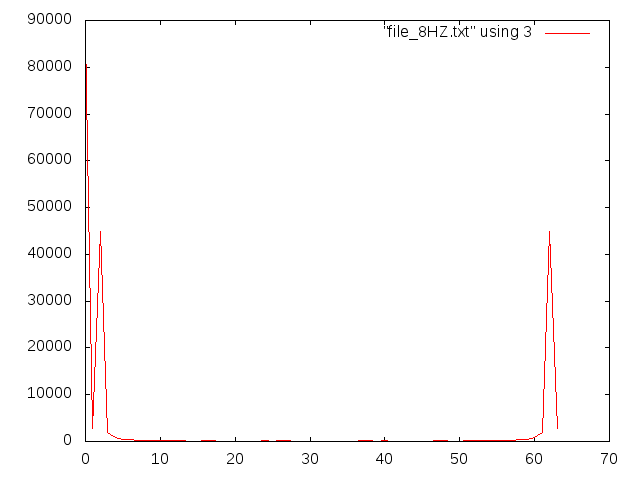
\includegraphics[width=0.9\textwidth]{output8HZ.png}
\caption{\label{fig:mesureDeSortie}Courbe des résultats de la FFT par l'entrée des donnés du Générateur basse fréquence}
\end{figure}

La FFT qu'on m'avait donnée était incorrecte, Giuseppe m'a donné un site Rosseta Code où on pouvait dénicher une FFT en langage C qui fonctionne. Je ne savais pas au départ utiliser la FFT, j'ai donc demandé à Giuseppe comment faire, il m'a dit que pour utiliser la FFT il fallait un tableau de donnée de courant et qu'après l'application de la FFT sur le tableau, le tableau représentait maintenant un tableau de donnée de fréquence.

Le but de cette tâche était de créer les bases de l'application simple pour ainsi réaliser un portage de l'application sur FreeRTOS. 

\subsection{ Programmation multi-threadée de l'ensemble sous FreeRTOS}

Pour effectuer cette tâche il me fallait connaître l'utilisation des threads, mais aussi celui des sémaphores de freeRTOS. 

il fallait mettre chacune des tâches dans un thread qui est une séquence d'instructions qui s'exécutent parallèlement aux autres threads. Tout en vérifiant que les tâches se font dans le bon ordre qui est convertisseur Analogique-Numérique puis la transformation par la FFT puis ensuite son écriture. L'exécution des tâches dans le bon ordre sera garanti par des sémaphores qui sont des objets permettant de protéger l'accès à une ressource par le biais d'un blocage si le sémaphore ne nous donne pas la main, ainsi un sémaphore du convertisseur Analogique-Numérique donne la main à la tâche de la FFT qui donne la main à la tâche de l'écriture sur la carte mémoire flash. Etant donné que l'ADC est une boucle sans fin il donne donc toujours quand il a fini une exécution du code de la FFT qui lui donne la main à une exécution du code de l'écriture dans la carte mémoire flash ainsi créant une périodicité. Là aussi on vérifie que les données concordes aux précédentes.

J'ai eu un problème avec les sémaphores, l'application ne s'effectuait qu'une seule fois par lancement du code alors que sans les sémaphores le code marchait en boucle, Julien m'a dit de faire un exemple simple pour voir ce qui ne marchait pas, j'ai remarqué que c'était la création du sémaphore qui faisait planter, la création par mutex avait un problème avec l'ordonnanceur que le binary n'avait pas. Comme j'écrivais sur un fichier pour ensuite le lire j'avais utilisé snprintf une fonction qui permet de mettre dans une chaîne de caractères à peu près ce que l'on veut, que j'utilisais pour mettre les résultats dans une chaîne de caractère avant de l'écrire, mais après que j'ai voulu mettre snprintf dans le code, il ne marchait plus. J'ai donc demandé à Julien Forget s'il n'avait pas une petite idée de ce qui posait un problème et il m'a dit que c'était probablement la taille de la pile des threads là où s'exécute les commandes, il se produisait certainement un overflow, il écrivait dans un endroit où il n'avait pas accès. Après avoir augmenté la taille des piles des threads ça marchait de nouveau.

Quand j'ai mis le code de Tilen Majerle pour le système d'exploitation de fichiers, surgit une erreur de conflit de timer, freeRTOS et le code de Tilen utilisait le même sur la carte STM32, en voyant des notes de Tilen j'ai pu définir un autre timer propre à son code sur la carte STM32 sans perturber celui de FreeRTOS. Quand le portage fut réglé et que la compilation s'exécutait correctement il eut des problèmes aux résultats le fichier étant sans droit et sans texte avec un nom sorti de nulle part. Le problème se situait à la fermeture du fichier étant donné que c'était une boucle infinie on ne pouvait pas fermer le fichier sans perturber l'exécution du code, j'ai dû créer une autre tâche qui fermait le fichier et stopper le code, car aucun intérêt à continuer si toutes les tâches ne s'exécutaient pas, au bout d'un temps qu'on définit, le fichier se ferme et donc permettait d'avoir les données de l'application et ces données concordent avec celle en baremetal.

Avec la représentation ci-dessous on peut voir quand les tâches se font et dans quel ordre. Ici l'ADC se déclanche 64 fois avant de donner la main à la FFT et pendant que la FFT se déclanche, l'ADC la préempte, après que la FFT s'est effectué elle donne la main à la FAT qui se fait préempter aussi par l'ADC. Dès que l'ADC se refait 64 fois avec les préemptions le cycle recommence, il donne la main à la FFT qui se fait préempter et après être terminé elle donne la main à la FAT. 

\begin{ganttchart}[inline,link mid = 0.4]{1}{25}
\gantttitle{Ordre d'exécution des taches}{25}\\
\ganttbar{Début de la préemption /fin du repos }{4}{19}\\
\ganttbar{ADC}{2}{7} 
\ganttbar{FFT}{9}{14}
\ganttbar{FAT}{16}{22}\\
\ganttbar{Fin de la préemption/début du repos de 4ms}{4}{19}
\ganttlink{elem0}{elem1}
\ganttlink{elem2}{elem0}
\ganttlink{elem3}{elem0}
\ganttlink{elem1}{elem4}
\ganttlink{elem4}{elem3}
\ganttlink{elem4}{elem2}
\end{ganttchart}


Après que l'application simple de traitement de signal on pouvait enfin la mesurer et savoir combien les tâches consomment. 


\subsection{Mesure de la consommation de l'application à l'aide l'Agilent N6705}

Pour effectuer les mesures de consommations on m'a donné un Agilent N6705, un analyseur de puissance, il possède quatre voies, un oscilloscope où on peut voir les courbes de chaque voie, courant, tension en fonction du temps, on peut régler pour chaque courbe son unité de mesure d'intensité ou de tension, on peut aussi changer l'offset qui est le point de départ de la courbe et aussi l'unité de mesure du temps, mais pour toutes les courbes. On peut allumer et éteindre les quatre voies ainsi que de choisir leurs intensités et leurs courants. On peut aussi programmer l'Agilent pour qu'il soit connecté par un câble Ethernet avec un ordinateur pour récupérer des données ou lui envoyer des scripts pour automatiser la configuration de l'Agilent.

Avec l'aide de Nadir Cherifi et de ses scripts, j'ai pu approfondir ma connaissance de l'Agilent N6705. Après avoir vu comment il utilisait ses scripts avec l'Agilent, j'ai dû mettre son code dans le projet puis compiler un programme existant avant que j'insère son code pour savoir s'il n'y avait pas de conflit entre son code et le projet, ensuite j'ai pu tester les tags de Nadir celui qui signale quand on entre dans une fonction et celui qui signale quand on en sort. Ainsi avec le lancement de ses scripts qui permettent l'allumage des deux voies de l'Agilent, la configuration de ces voies, l'exécution du code de la carte STM32 pendant un certain temps et avec une période de réception des données par l'Agilent, ces mesures qui seront transmises dans l'ordinateur par un câble Ethernet configurer par un des scripts et une visualisation du graphique reçu ainsi que les temps de départ et de fin de chaque tâche ainsi que sa consommation reçue par l'usart. 

J'ai pu utiliser les tags de Nadir Cherifi dans l'application simple de traitement de signal pour pouvoir lancer les mesures, avec les résultats de ses mesures, Julien Forget et Giuseppe Lipari m'ont dit qu'il y avait une préemption qui est la capacité d'un système d'exploitation multi-tâche d'interrompre une tâche en cours en faveur d'une tâche de priorité supérieure, mais que c'était prévisible pour du temps réel.

J'ai pu tester les scripts de Nadir Cherfi, il me donne la courbe de la consommation d'énergie de l'exécution du code, sur la figure ~ref{fig:resGraph} on peut voir une courbe rouge qui est la consommation du code chargé sur la carte STM32, on peut voir aussi des lignes verticales qui représente un tag d'entrée ou un tag de sortie inséré dans le code chargé.

\begin{figure}[H]
\centering
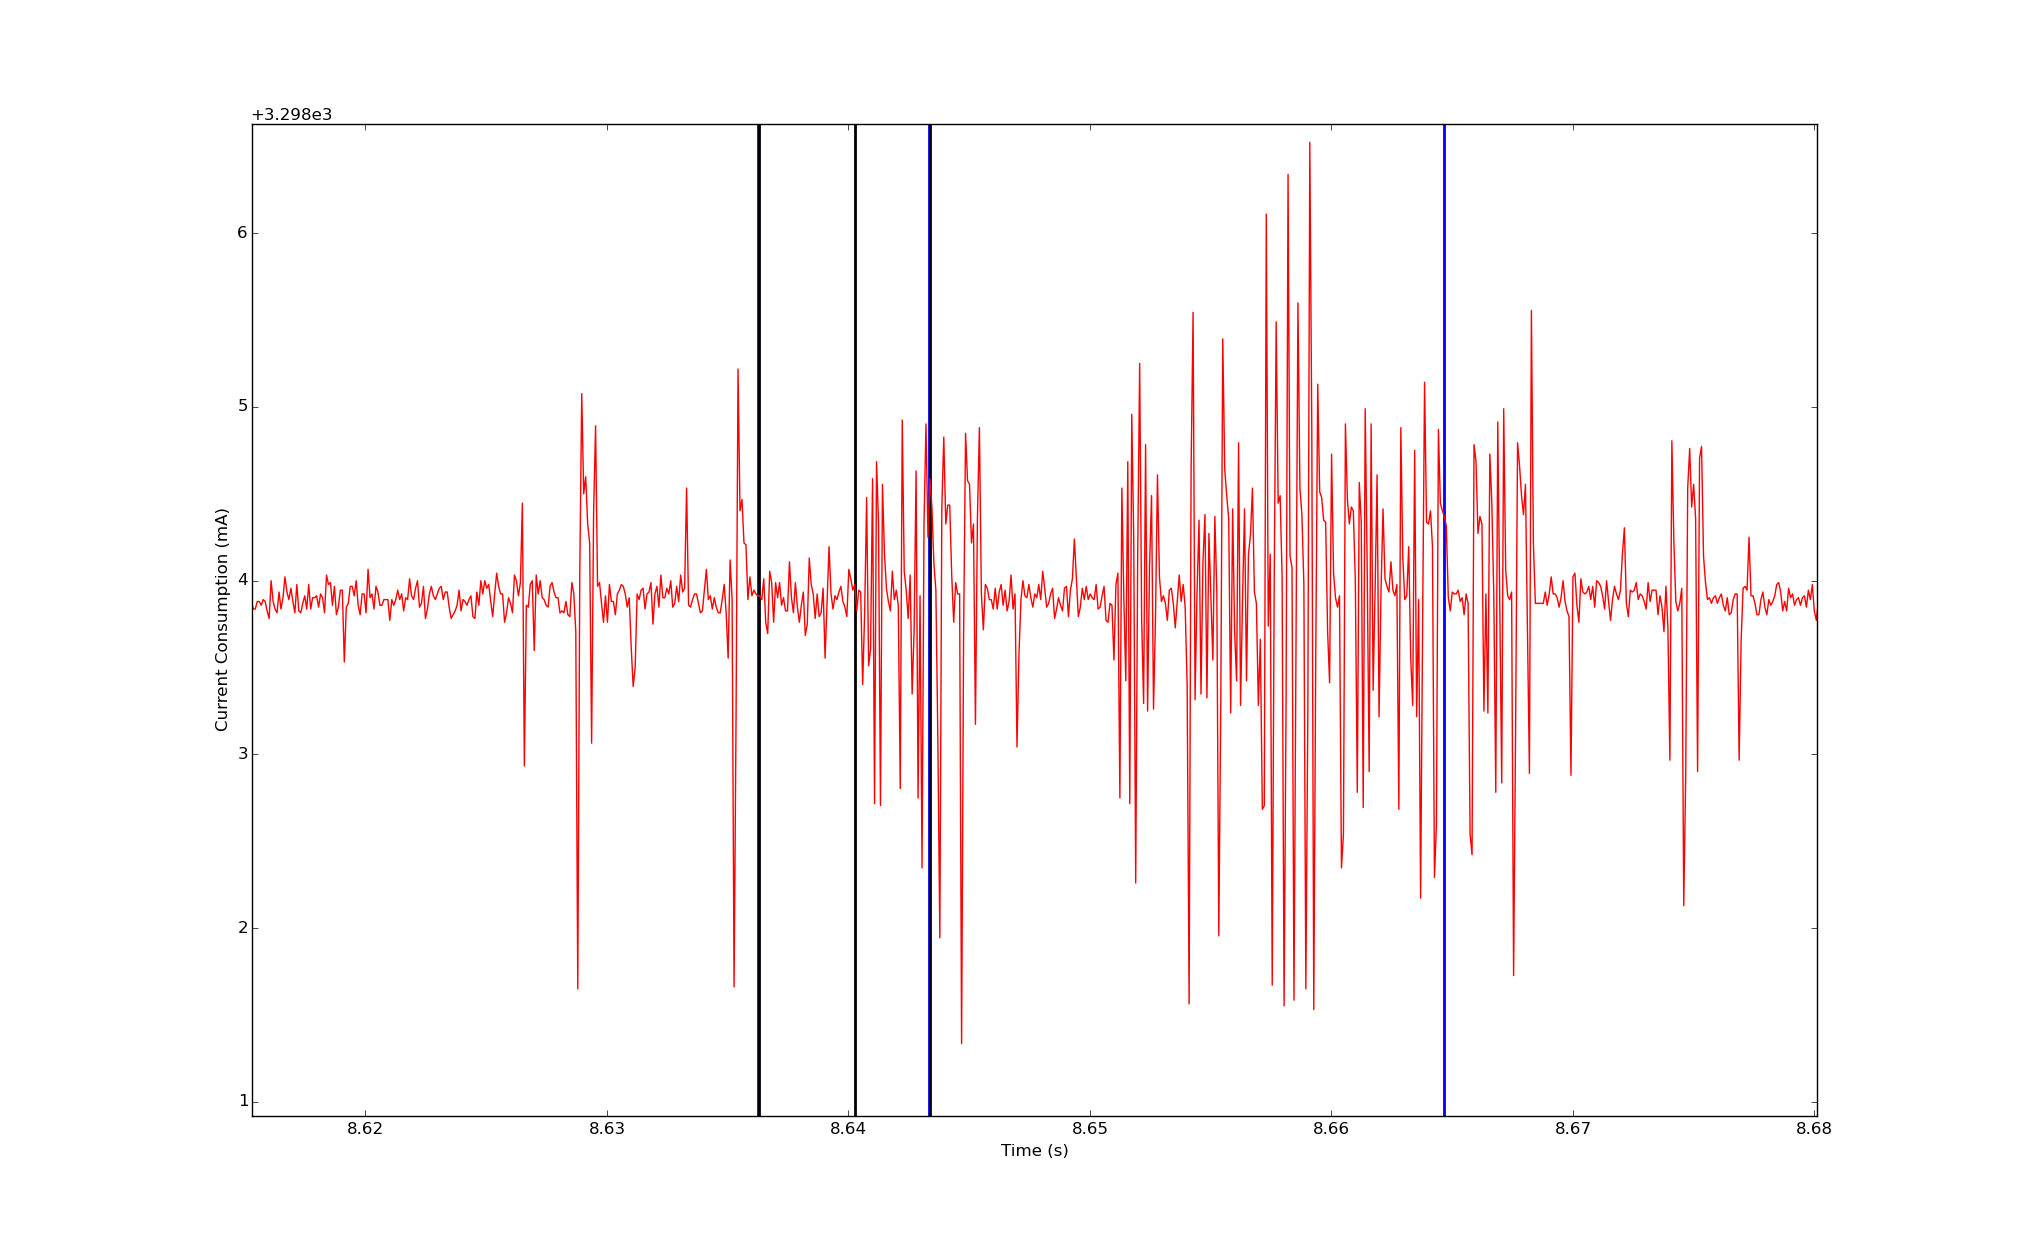
\includegraphics[width=0.9\textwidth]{figure_2.png}
\caption{\label{fig:resGraph} Courbe résidant du code modifié et des scripts de Nadir}
\end{figure}

Il fallait une autre exécution de mesure que les scripts de Nadir Cherifi, il fallait donc montrer quand les tâches se déclenchaient sur l'Agilent, pour ce faire on pouvait recourir à trois GPIO, pattes d'entrée et de sortie de la carte STM32, une pour chaque tâche nous pouvons savoir quand la tâche s'exécute et quand elle s'arrête, en déclenchant la GPIO au départ de la tâche puis en la désactivant à la fin, seulement comme la mesure de temps d'une conversion Analogique-Numérique était trop rapide l'Agilent ne pouvait pas l'indiquer avec la GPIO, j'ai décidé de prendre la mesure de tous les échantillons de conversion au lieu d'un seul.

On peut voir le résultat donné par le code et les scripts associés aux GPIO, on remarque que chaque fois qu'on a un pic montant pour les courbes concernant les tâches cela équivaut au commencement de la tâche et qu'à chaque pic descendant à la fin de cette tâche. On peut donc correspondre chaque intervalle d'un pic montant à un pic descendant une tâche. Sur la figure~ref{fig:myResGraph}, on peut voir la courbe rouge qui est la consommation du code chargé ainsi que trois autres courbes, ces courbes sont les courbes créent par les GPIO. On peut distinguer trois courbes de GPIO, une pour chaque tâche, on voit que l'ordre ADC FFT FAT est conservé et qu'il y a bien une préemption de l'ADC pendant que la FFT ou la FAT est active, car on voit un pic descendant de l'ADC qui donne la main à la FFT, mais qui par la suite la reprend dès qu'il finit sa pause de 4ms, dès qu'il finit de s'exécuter redonne la main à la FFT, après que la FFT s'est effectué la courbe à un pic descendant et ne se remonte pas avant un nouvel appel de l'application. On remarque la même chose pour la FAT que la FFT. On peut voir sur le schéma une consommation linéaire de l'ADC qui est à peu près une consommation au repos des tâches, car il s'exécute rapidement, mais aussi que pendant la FFT et FAT le code consomme plus, on peut remarquer que la consommation de la FFT est assez régulière, mais celle de la FAT ne l'est pas. On remarque que la tâche de l'ADC consomme le moins, celle de la FFT consomme un peu plus et celle de la FAT consomme le plus en moyenne.

\begin{figure}[H]
\centering
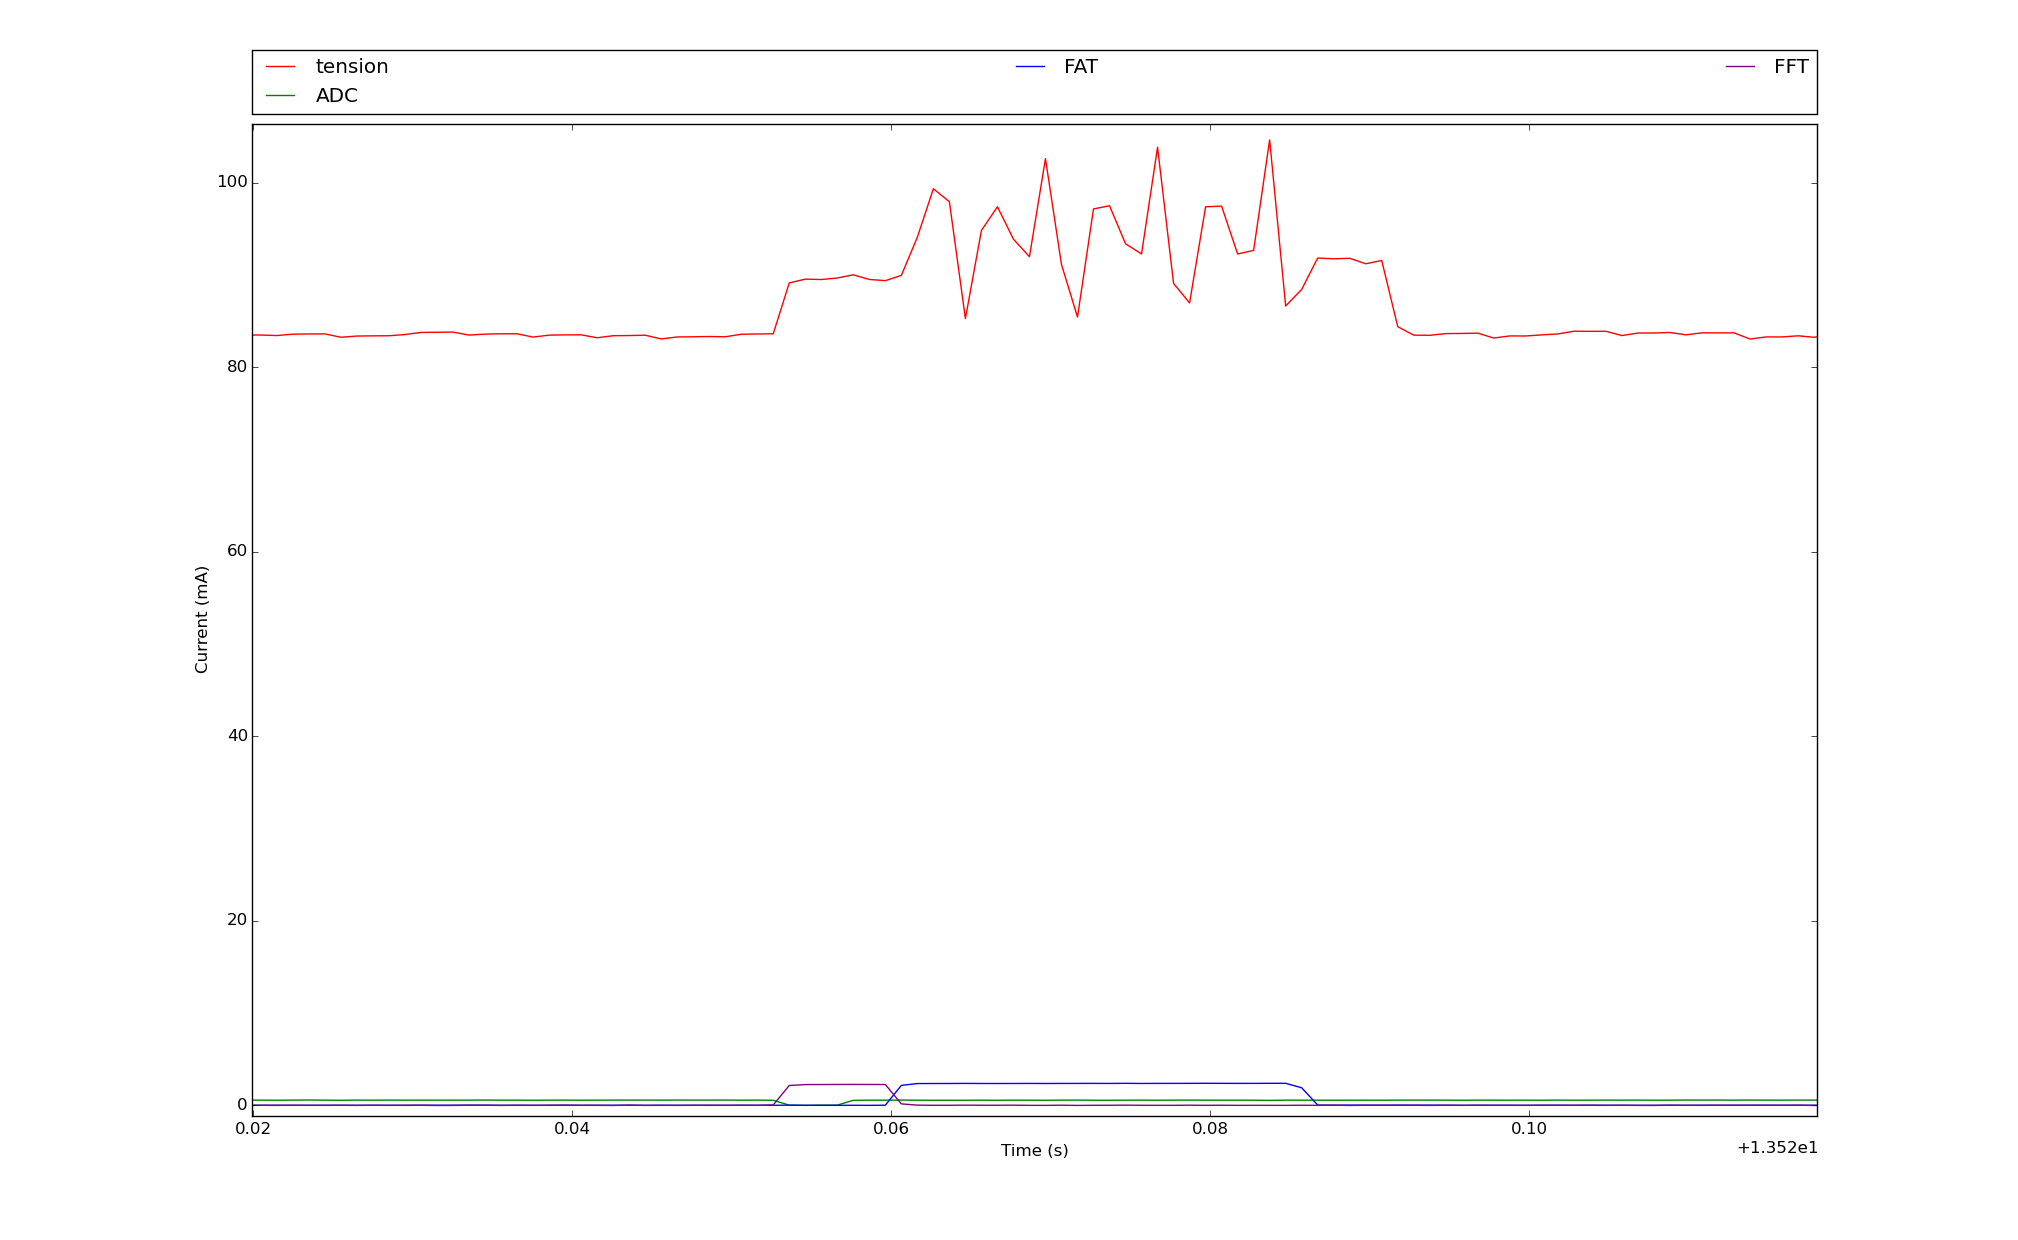
\includegraphics[width=0.9\textwidth]{resultat_2.png}
\caption{\label{fig:myResGraph} Courbe résidant du code avec les trois GPIO}
\end{figure}

La mesure étant possible et les scripts automatisant tout il ne restait plus qu'à changer les fréquences du processeur, des tâches et périphériques pour voir ce que ça change niveau consommation d'énergie. 


\section{Conclusion}

\subsection{Perspectives}

\subsubsection{Expérimentation sur les possibilité de variation de fréquence sur la STM32 concernant le processeur et les périphériques}

Pour savoir la consommation d'énergie change quand je modifie la fréquence des périphériques, je vais devoir modifier mon code pour pouvoir facilement modifier la fréquence des périphériques dans l'initialisation des périphériques.

Après avoir fait ces changements, je vais devoir trouver les limites de fréquence, par exemple si la conversion Analogique-Numérique a une fréquence trop faible ce qui augmentera son temps d'exécution grandement et si c'est suffisant pour qui ne laisse pas une préemption donc ne laissera pas la main ni à la FFT ni à la FAT, il n'y aura que lui qui s'exécutera donc aucun intérêt de mesurer dans ce cas-ci.

Après cette tâche on pourra étudier les variations de la consommation, selon les différents changements de fréquence.

\subsubsection{Etude des variations de la consommation, selon le changement de fréquence}  

Avec les modifications de fréquence, on va pouvoir étudier la variation de la consommation de l'application simple de traitement de signal par le changement des fréquences, celles des tâches, celle du processeur ou encore celle des périphériques.

Après avoir fait une dizaine de fois pour chaque changement de fréquence pour ainsi avoir une moyenne et donc empêcher d'avoir des résultats qui auraient varié à cause d'autre chose que le changement de fréquence. Grâce à ces résultats on va pouvoir déterminer quel périphérique consomme le plus et à quelle fréquence. 

\subsection{Les apports du stage}

Ce stage m'a apporté non seulement de diverse connaissance en informatique jusque là inexploré par moi, mais aussi comment se passe un métier dans la vie active mais également le métier de chercheur et la rencontre d'un lieu de recherche actif avec des doctorants, des thésars et des chercheurs.

Dans les compétences que ce stage m'a apporté :

La compréhension d'une carte STM32 ainsi comment coder un morceau de code et l'utilisation de quelques-uns de ses périphériques comme la carte mémoire flash, un convertisseur Analogue-Numérique, un usart en port série, l'approche d'un os minimaliste, l'appréhension d'une FFT, l'utilisation d'un Agilent N6705 un analyseur de puissance ainsi qu'un générateur de basses fréquences ainsi qu'une BreadBoard. 

\subsection{Compétences acquises}
\begin{enumerate}
\item{Comprendre comment fonctionne une carte STM32 (Branchements + Code)}
\item{Savoir utiliser une FFT}
\item{Savoir manipuler une carte flash}
\item{Savoir utiliser un Aglient N6705A}
\end{enumerate}



\section{Résumé du stage en anglais}

\subsection{ Presentation}

The Institute for Research in Hardware and Software components for Information and Advanced communication (IRCICA) associate the CNRS (National Research Center for Science) with Lille1 University.It brings together nearly 120 members from 4 different

laboratories. Here are several research themes:

    Human-machine interfaces ;
    Sensor networks ;
    Photonics ;
   Bio-inspired architectures.
    
    
\subsection{ My mission }
I had to measure the consumption (CPU and peripherals) of an embedded board to know what consumes the most and how to optimize its code to consume less, with a simple example of signal processing application that I have program. Initially I had learnt to use the STM32F4-discovery card, to create a simple signal processing application and to write results on flash memory cards. Thanks to Nadir Cherifi's help, a PhD student, I was able to write data in flash memory card with a file system (FAT). Then,i took a  set of sample of entries of one of the card input pins connected to a low frequency generator for conversion, using FFT (fast fourier transform) in frequency. After checking the accuracy of the application results, we will finally be able to measure consumption of each differed mode task with a time marker so that we have a precise to know which task is begin carried out, when, and what the quantity of energy that is used it is then possible to deduce what consumes the most (indeed, these landmarks should not change the code execution in its entirety, and not changing his energy consumption or his running time).


\subsection{ Technologies used} 
I worked on a traditional Debian machine programmed for a STM32F4 Discovery card, and used an Agilent N6705 to measure energy consumption. To automate power measurements, i employ
Python scripts provided (like scripts Run) or modifed to match my expectations. The embedded code was in C, through STM microelectronics library that provides many features for ease the interaction with the material, I used a FAT that is a file system to write and read in Flash memory. I also used the utilities specifically designed for programming on ARM target: mainly GCC for compilation. Finally used a minicom for receiving and reading the output from the card.
\subsection{ Conclusion}

This internship introduced me to embedded systems and the work of researchers and PhD students. It was hard to start from scratch but after a few uses of the card, I reached a better understanding of what to do. I got familiar with electronics. I also did some personal tests such to calculate as to check the difference in speed and consumption of what we learn in advance system programming course.

\section{Mots clés}

\begin{enumerate}
\item ADC: Convertisseur Analogue-Numérique, il sert à prendre et convertir une donnée sur un canal d'ADC sur la carte STM32.  
\item Agilent : Un analyseur de puissance pour mesurer la consommation. 
\item BreadBoard : Permet de faire des schémas d'électroniques sans à avoir à souder les composants ensemble.
\item Burn : Commande pour envoyer le code sur la carte.
\item Carte mémoire flash : Une carte où on écrit ou lit des données.
\item FAT : Système d'exploitation de fichier.
\item FFT : Fast Fourier Tranformation, sert à convertir des données de courant en données de fréquence. 
\item GBF, générateur basses fréquences qui permet d'alimenter avec un courant et d'une fréquence donnée. 
\item Makefile : un fichier qui s'occupe des dépendances des fichiers écrits en un langage d'informatique.
\item Pattes d'entrée de STM32F4-discovery : Sert de port d'entrée ou de sortie de la carte STM32
\item préemption : c'est la capacité d'un système d'exploitation multi-tâche d'interrompre une tâche en cours en faveur d'une tâche de priorité supérieure
\item Sémaphore : Un objet permettant de protéger l'accès à une ressource. 
\item Thread : Une séquence d'instructions qui s'exécutent parallèlement aux autres threads
\item STM32F4-discovery : La carte où on introduit le code à exécuter.

\end{enumerate}

\end{document}
